%%%%%%%%%%%%%%%%%%%%%%%%%%%%%%%%%%%%%%%%%%%%%%%%%%%%%%%%%%
%   Autoren des Abschnitts:
%   Jakob Kautz
%   Olivier Stenzel
%%%%%%%%%%%%%%%%%%%%%%%%%%%%%%%%%%%%%%%%%%%%%%%%%%%%%%%%%%

% !TEX root =  master.tex
\graphicspath{ {./img/} }

\chapter{Konzeption - Hardware}\label{Hardware - Konzeption}~\nocite{*}

Für die Umsetzung eines selbstspielenden Klaviers wurden verschiedene technische Überlegungen angestellt.
Die Grundfragen, welche bei der Konstruktion auftraten, betrafen die Auswahl und Implementierung der
Aktuatoren, die Methode des Anspielens der Klaviertasten sowie die Signalübertragung des Arduinos.
Im Hinblick auf die Aktuatoren muss eine präzise Steuerung der Tasten
ermöglichet werden, ohne dass Genauigkeit und Geschwindigkeit des Anspielens vernachlässigt werden.
\newline
Dafür werden diese mit den Klaviertasten verbunden, um die mechanische Integrität des Klaviers
zu erhalten und gleichzeitig eine präzise Steuerung zu gewährleisten.\newline
Die Signalübertragung erfolgt über einen Mikrocontroller.
Da der gängige Mikrocontroller i.d.R. nicht über ausreichende Ausgänge verfügen,
um alle Tasten anzusteuern, müssen diese erweitert werden.
Eine solche Erweiterung (siehe Kapitel \ref{output}) ermöglicht es, alle 88 Tasten des Klaviers anzusteuern.

\section{Mechanik}\label{vorgehenHW}

\subsection{Auswahl des Klaviers}

Da sich dieses Projekt nicht auf die theoretische Konzeption beschränkt, muss ein entsprechendes Testobjekt - ein reales Klavier - gefunden werden.
Dieses muss einige Voraussetzungen erfüllen:
\begin{enumerate}
	\item 	Der Preis muss im Rahmen des selbst gestellten Budgets (< 2000 €) liegen
	\item 	Es muss leicht auseinander zu bauen sein, um die Mechanik zugänglich zu machen
	\item 	Es muss vollständig sein (alle 88 Tasten)
	\item 	Es muss stimmbar sein
	\item 	Der Transport muss einfach durchzuführen sein
\end{enumerate}


\subsection{Ansteuerungskonzept} \label{konzeptionHW-ansteuerungskonzept}
Beim Ansteuerungskonzept der Tasten muss auch beachtet werden, wo die Magnete befestigt werden.

//Drücken der ziehen, oben oder unten...
1. Oben
Klavierhand
Schiene
Aufsatz mit 88 oben drüber
2. unten
ziehen
drücken

\subsection{Aktuator}\label{subsec:aktuator}

Schrittmotor, Hubmagnete, etc.

\subsection{Verbindung Tasten und Aktuatoren}

Wie in Kapitel \ref{konzeptionHW-ansteuerungskonzept} beschrieben wurde sich für ein Ziehen der Tasten entschieden.
Dieses Ziehen wird technisch mittels Hubmagneten umgesetzt.
In diesem Kapitel wird ein Konzept ausgearbeitet, welches beschreibt wie und wo die Hubmagnete am Klavier und den Tasten befestigt werden.
Zusätzlich wird der Aufbau bezüglich Reibung und Akkuratheit weiter verbessert.
\newline
Die Grundidee ist, eine Schnur, oder Ähnliches, mittels eines waagerechten Loches in der Taste, an dieser zu befestigen.
Anschließend wird jede Schnur jeweils durch ein senkrechtes Loch im Klaviaturbalken (bzw. Tastenbrett), worauf die Tasten liegen, in den Fußraum geführt.
Damit die Pianist:innen nicht durch Platzmangel im Beinbereich eingeschränkt sind,
werden die Seile entlang der Verkleidung zur unteren Frontplatte des Klaviers geführt.
Dort werden die Hubmagnete in zwei Reihen über die gesamte Breite befestigt.
Um die Intensität des Tastendrucks zu steuern und die Durabilität des Materials zu verlängern, sollte die Reibung am Seil möglichst gering gehalten werden.
Dazu werden mittels Rohren, welche waagerecht unter dem Klaviaturbalken entlang der Löcher montiert werden, die Seile umgelenkt.

\textit{Organisation der Aktuatoren}

Die Idee ist, die Hubmagnete entlang der Klaviatur zu befestigen, um die Tasten möglichst senkrecht nach unten ziehen zu können.
Hierfür müssen folgende Aspekte berücksichtigt werden:

begin{itemize}
	\item Breite der Hubmagnete
	\item Hitzeentwicklung
	\item Seilführung
	\item Stabilität
	\item Modularität
end{itemize}

Ein Hubmagnet hat die Maße 2,5 cm x 6 cm.
Das Tastenbrett für 88 Tasten ist allerdings nur 140 cm breit, wodurch pro Tastenansteuerung nur ca. 1,6 cm zur Verfügung stehen.
Bildet man zwei Hubmagnetreihen übereinander, hat jede Tastenansteuerung 3,20 cm Platz.

Durch die 7mm Abstand ist eine Wärmeabfuhr über die Luft in geringem Ausmaß möglich.
Ob dies ausreicht, muss in späteren Tests (siehe Kapitel \ref{tests}) ermittelt werden.

Alle Seile werden pro Hubmagnetreihe, parallel zwischen Tasten und Hubmagnete verbunden.

Die Hubmagnete direkt unter dem Tastenbrett zu befestigen wäre eine triviale Lösung würde allerdings auf Kosten der Stabilität und Funkionalität gehen.
Deshalb werden die Hubmagnete am Corpus des Klaviers (untere Frontplatte) befestigt.

Um die Austauschbarkeit der Komponenten zu verbessern, werden die Hubmagnete nicht direkt an der unteren Frontplatte,
sondern auf zwei Pressspanplatten (ca. 70 cm x 25 cm) befestigt, welche an vier Punkten mit dem Klavier verschraubt werden.

*Bild von Brett-Sikzze

\textit{Optimierung der Seilführung}

Würde man den Aufbau so belassen, hätte man deutliche Hub-Verluste und könnte unter Umständen die Tasten nicht mehr ausreichend betätigen.
\newline
Dies kann man auch mathematisch beweisen:
\newline geg.:
\newline Strecke bis zur ersten Reihe Hubmagnete h1 = 17 cm
\newline Strecke bis zur zweiten Reihe Hubmagnete h2 = 27 cm
\newline Strecke bis zu den schwarzen Tasten t1 = 12 cm
\newline Strecke bis zu den weißen Tasten t2 = 18 cm

\newline Seil zur schwarzen Taste im entspannten Zustand ht1_{entspannt}
\newline Seil zu den weißen Tasten im entspannten Zustand ht2_{entspannt}

\newline ht1_{entspannt} = $\sqrt {h1^{2} + t1^{2}}$ = 20.81 cm
\newline ht2_{entspannt} = $\sqrt {h2^{2} + t2^{2}}$ = 32.45 cm

\newline ht1_{gespannt} = $\sqrt {(h1 + 1) ^{2} + t1^{2}}$ = 21.63 cm
\newline ht2_{gespannt} = $\sqrt {(h2 + 1)^{2} + t2^{2}}$ = 33.29 cm

Die Differenz zwischen ht1_{gespannt} und ht1_{entspannt} (bzw. ht2) beschreibt die Tiefe, die eine Taste gedrückt werden kann.
\newline Diese beträgt 0.82 cm, bzw. 0.84 cm.

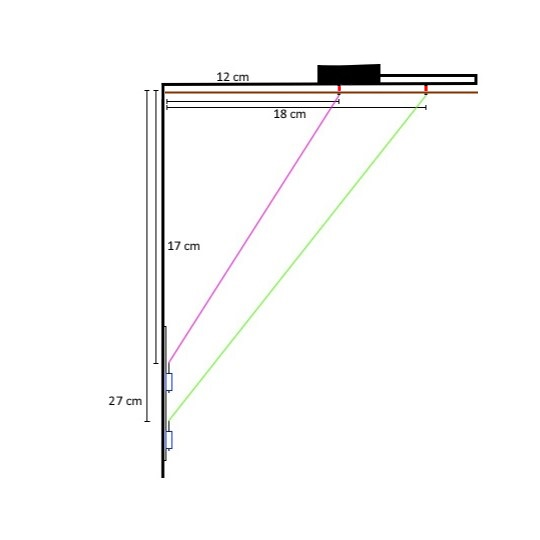
\includegraphics [width=8cm, height=10cm] {img/Umlenkung_locker}\caption{Taste locker ohne Umlenkung}
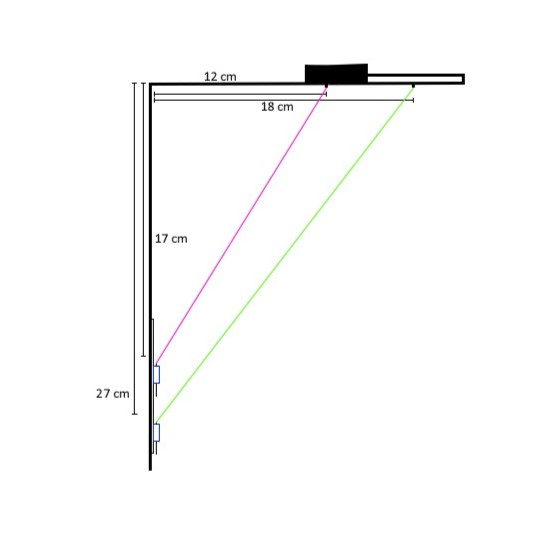
\includegraphics [width=8cm, height=10cm] {img/Umlenkung_gezogen}\caption{Taste gezogen ohne Umlenkung}

Mittels einer Umlenkung (PVC-Rohr) werden die Seile so geführt, das sie senkrecht auf die Hubmagnete fallen.
Somit wurde die Tiefe, mit der die Taste gedrückt werden kann wieder auf annähernd 1cm erhöht werden.

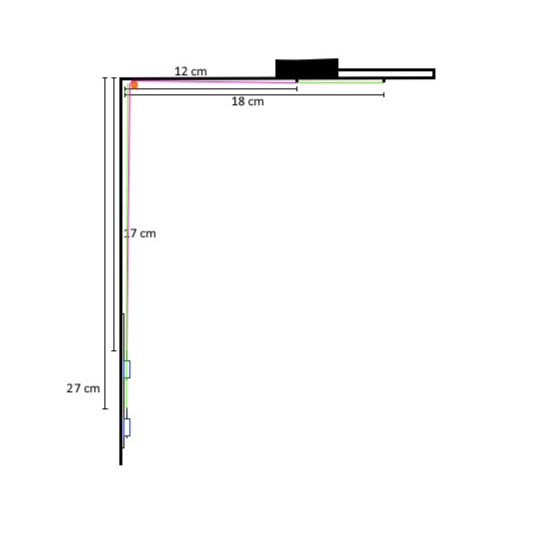
\includegraphics [width=8cm, height=10cm] {img/mitUmlenkung_locker}\caption{Taste mit Umlenkung}


\textit{Auswahl des Seils}

Wie eben erwähnt wird das Ziehen durch ein Seil ermöglicht.
Dafür wird ein leichtes, formbares und dehnungsresistentes Material benötigt, da die eine Seite mit dem Hubmagnete und die andere durch ein Loch in der Taste verknotet werden sollt.
Je leichter das Material ist, desto weniger wird die Genauigkeit der Kraftübertragung zwischen den Magneten und den Tasten verändert.
Durch die Formbarkeit kann der Knoten sehr eng an der Taste geschnürrt werden, wodurch das Ansprechverhalten schneller erfolgen kann.
Da die Anschläge ruckartige Bewegungen sind, ist es wichtig ein dehnungsresistentes Seil zu verwenden.
Würde sich das Seil dehnen lassen, würde ein Teil der Kraft nicht bis zur Taste gelangen und somit den Anschlag abschwächen.

\subsubsection{Nähgarn}

Als Erstes wurden Nähgarn, welches zur Hand war getestet.
Auch doppelt verlegt hielt es der ruckartigen Ziehbewegung mit 25N des Hubmagnetens nicht stand.
Vier Fäden funktionierten zu Beginn gut, leierten allerdings schnell aus.

\subsubsection{Nylonsaiten}

Als Nächstes wurde die g-Saite einer Gitarre verwendet.
Durch den höheren Durchmesser und das stärkere Material riss und leierte die Saite nicht aus.
Da die Saite kaum Flexibilität liefert, war die Befestigung an der Taste äußerst schwierig.
Beim Ziehen des Magnetes wurde erst die lockere Schlaufe an der Taste gestreckt, wodurch nicht der vollständige Hub des Magnetes auf die Taste übertragen werden.

\subsubsection{Angelschnur}

Aus Erfahrungen aus dem Angelbereich konnte schnell eine geeignetere Schnur gefunden werden.
Genauer handelt es sich um eine geflochtene Schnur aus Polyethylene.
Mit einem Durchmesser von 1.6mm ist sie nicht nur sehr dünn und flexibel, sondern kann auch bis zu 7kg standhalten.
Auch nach ausgiebigem Testen erfüllt die Angelschnur die Anforderungen.
Damit ist nun auch das Spielen des Forellenquintetts von Schubert ein leichtes.

\subsection{Klangdämpfung der Aktuatoren}
Die Hubmagnete machen beim Anschlagen laute "klack" Geräusche, welche von der Melodie des Klaviers ablenken.
Genauer handelt es sich um das den Metall-Anker, der gegen das Ende des Metall-Gehäuses stößt.
Auch hierfür gab es mehrere Ideen und Tests, um das Geräusch zu dämpfen:

\subsubsection{Isolierfolie}

Die erste Überlegung war die Auskleidung des Innenraums der Hubmagnete mit Isolierfolie.
Diese Idee wurde wieder verworfen, da das Wissen über die Hitzeentwicklung zu diesem Zeitpunkt noch zu gering war, um sicherzustellen, dass die Isolierung dem standhält.

\subsubsection{Gummi-Stopper}

Die nächste Idee war das Limitieren des Schlags durch Gummiringe (Dichtungsringe) zwischen Anker und dem äußeren Gehäuse.
Da für die Befestigung keine zufriedenstellende Lösung gefunden wurde, wurde auch diese Idee verworfen.
zurück schellen zu hoch, als dass wir die Klangdämpfung umsetzen würden.

Notiz von Oli: Motorlager verwenden zwischen Platte und Klavier
Notiz von Oli:
Aktuatoren Geräuschreduzierung Tests:

Weg normal: 10mm

\subsubsection{Schaumstoff}

*siehe bild
Wie im Bild zu sehen wurde die "Gummi-Stopper"-Idee leicht mit Schaumstoff leicht verändert.
+ Das Klopfgeräusch konnte vollständig verhindert werden.
- Durch den Schaumstoff kann 1mm Hub nicht verwendet werden, weshalb nur noch 9mm übrig bleiben.
- Außerdem ist der Aufbau optisch nicht ansprechend.


\subsubsection{Seil (2mm Durchmesser) um den Anker}

Um das "Problem" der schlechten Ästetik beim Schaumstoff zu beseitigen, wird nun ein 2mm dickes Seil im Inneren des Gehäuses um den Anker gewickelt.
+ Auch hier konnte das Klopfen vollständig beseitigt werden
+ Von außen sieht man keine Veränderung
+ Bezogen auf die Hitzeentwicklung scheint das Seil nach den bisherigen Tests gut Stand zu halten.
- Durch die Dicke des Seils, werden 2mm Hub nicht verwenden, weshalb nur noch 8mm übrig bleiben.


\section{Elektronik}\label{Vorgehen - Hardware}


\subsection{Mikrocontroller}\label{Ansteuerung}
Um die Signale des Programmes an die Aktuatoren weitergeben zu können, wird ein Mikrocontroller benötigt.
Auf dem Markt steht eine hohe Anzahl an Mikrocontrollern zur Verfügung, wobei für diese Arbeit ein Arduino und ein
Rasperry Pi betrachtet wurden (Wobei es sich bei einem Rasperry Pi genau genommen um einen Einplatinencontroller
handelt). \newline

%Arduino Intro
\begin{minipage}{0.7\textwidth}
	\paragraph{Arduino}
	Bei einem Arduino handelt es sich um eine Plattform für die Entwicklung von elektronischen Prototypen. Er besteht aus
	einem Mikrocontroller-Board, das mit verschiedenen Sensoren, Aktuatoren und anderen elektronischen Komponenten
	verbunden werden kann. Der Arduino verfügt über digitale und analoge Ein- und Ausgangspins, die für die Interaktion mit
	externen Geräten verwendet werden können.
\end{minipage}
\begin{minipage}{0.3\textwidth}
	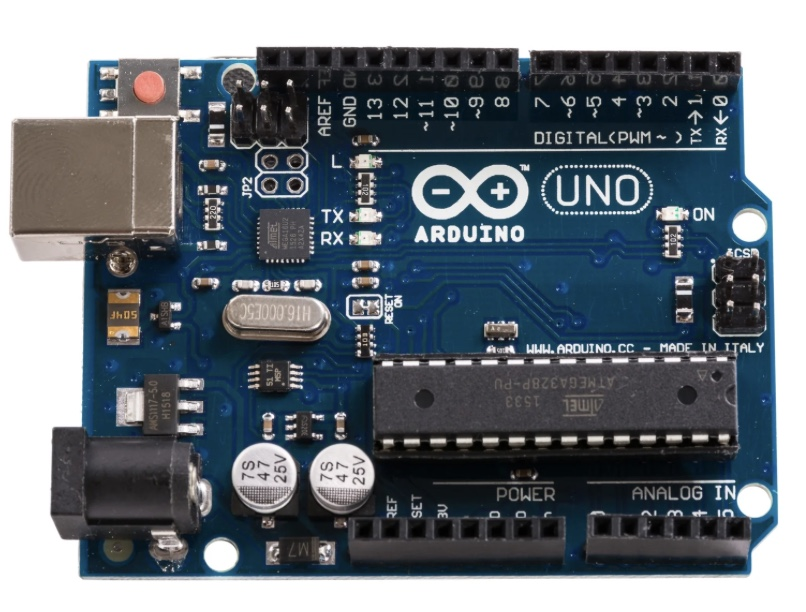
\includegraphics [width=\textwidth] {img/ArduinoR3}
\end{minipage}
\newline

%Pi Intro
\begin{minipage}{0.3\textwidth}
	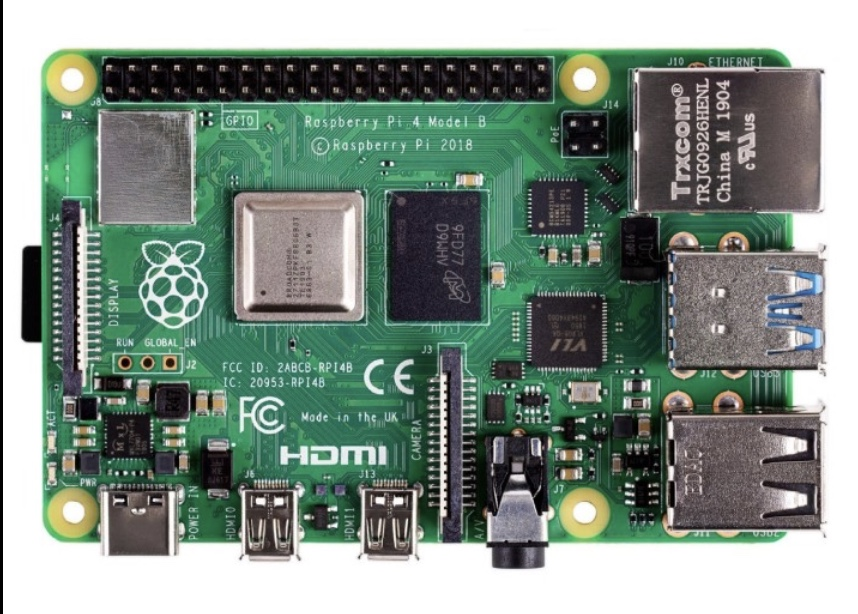
\includegraphics [width=\textwidth] {img/RasperryPi}
\end{minipage}
\begin{minipage}{0.7\textwidth}
	\paragraph{Rasperry Pi}
	Ein Rasperry Pi ist ein Einplatinencontroller, der auf einem ARM-Prozessor basiert. Er ist dafür konzipiert, eine breite
	Palette von Anwendungen zu unterstützen, von Prototypenbau bis IoT.
	Im Gegensatz zum Arduino verfügt er über einen Prozessor und ist besonders für komplexe und Rechenlastige
	Projekte geeignet.
\end{minipage}
\newline

%Vergleich
Die Entscheidung für den verwendeten Mikrocontroller traf auf den Arduino. Der Rasperry Pi stand vor allem aufgrund
seiner höhere Speicherkapazität und Rechenleistung zur Diskussion, wodurch eine Komplexe Ansteuerungslogik
möglich ist und ein Großteil des Programmes auf dem Rasperry Pi ausgeführt werden kann. Allerdings ist er aufgrund
seines Betriebssystems und einer erhöhten Latenz nicht für Echtzeit-Anwendungen bzw. Geschwindigkeitskritische
Anwendungen ausgelegt. Im Gegensatz dazu bietet der Arduino eine Echtzeitverarbeitung mit geringer Latenz.
Außerdem verfügt ein Arduino über eine recht simple Hardware-Interaktion - er ist darauf spezialisiert, die
Hardware direkt anzusprechen und ist somit besser für Projekte geeignet, welche eine präzise Ansteuerung von
Aktuatoren benötigt. Zudem ist die Komplexität der Ansteuerung nicht so hoch, dass der Microcontroller über eine
hohe Rechenleistung verfügen muss. \newline
Für das Projekt wird spezifisch ein Arduino R3 verwendet. Bei der Auswahl des spezifischen Arduinos wurden der Arduino
Uno, Nano und R3(auch: mega 2563) betrachtet. Im Prinzip wäre jedes der Modelle für die Anwendung möglich, allerdings
verfügt der R3 im Gegensatz zu den anderen beiden Modellen über mehr Speicherkapazitäten (256KB Flash Speicher
gegenüber der 32KB vom Arduino Uno und den 16KB des Arduino Nanos). Der Arduino Uno verfügt zwar über mehr Ports,
allerdings bringt dies keinen Mehrwert, da die Anzahl der benötigten Ausgänge auch bei einem Arduino Uno nicht erreicht werden
(siehe Kapitel~\ref{output}).
Der Arduino R3 bietet - wie die anderen beiden Modelle auch - PWM (Pulsweitenmodulation) Pins, die im Rahmen des Projekts
genutzt wurden.

\subsection{Pulsweitenmodulation (PWM)}\label{PWM}
Oftmals ist bei der Ansteuerung nicht die gesamte Versorgungsspannung erwünscht bzw. gebraucht. In diesen Fällen muss
die anliegende Spannung varriiert werden, damit die Spannung am Ziel dem gewünschten Wert entspricht.
Angenommen es ist eine Spannung von 2.5V erwünscht, wobei die Vollversorgungsspannung 5V beträgt. Das Signal kann
dafür die Hälfte der Zeit ausgeschaltet werden, womit zwischen 0V und den vollen 5V durchschnittlich insgesamt 2.5V
anliegen. Wenn die Frequenz zwischen an- und ausschalten des Signals erhöht wird, desto weniger wird diese ``künstlich''
simulierte Halbierung wahrgenommen. \newline
PWM bedient sich im Grunde genau dieser Technik.
Einfach ausgedrückt, wird die Zeitdauer eines digitalen Signals variiert wird, um einen
durchschnittlichen Wert zu erzeugen. Bei den PWM- Ausgängen wird die Pulsweite - die Dauer der Einschaltzeit -
des Signals angepasst, um die gewünschte Spannung zu erreichen. \newline
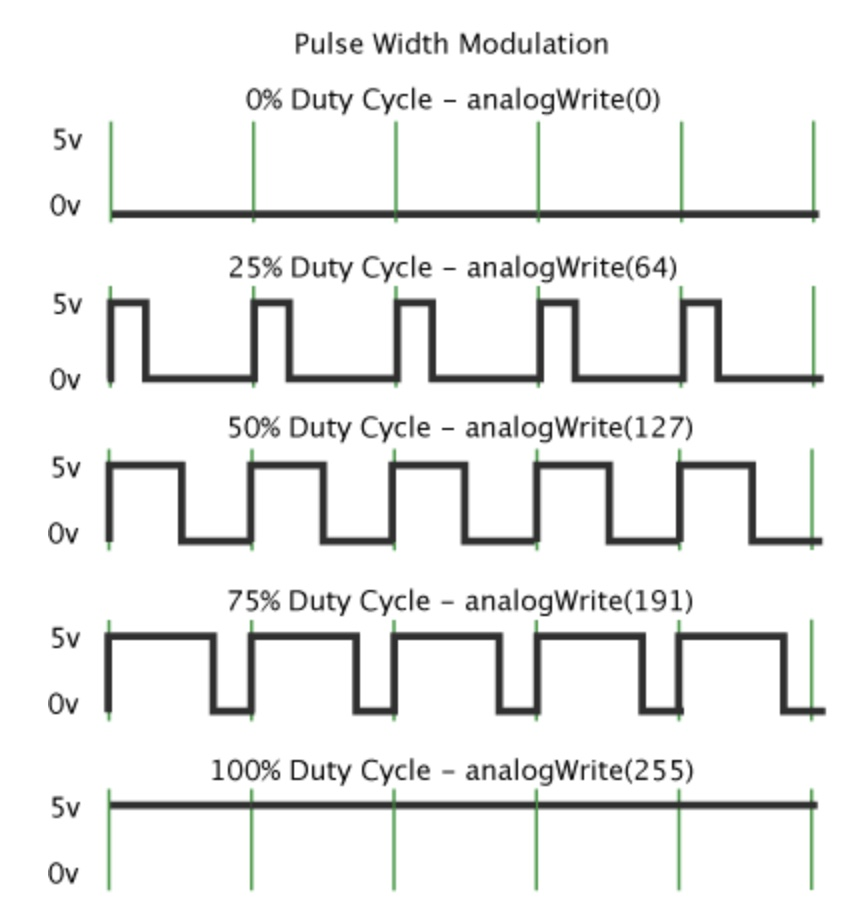
\includegraphics [width=13cm, height=8cm] {img/pulsweite} \newline \newline
Spezifischer ausgedrück passiert folgendes:
Eine Digitale Steuerung wird verwendet, um eine Rechteckwelle - ein Signal das zwischen Ein und Aus umgeschaltet wird
- zu erzeugen. Dieses Ein-Aus-Muster kann Spannungen zwischen der vollen Versorgungsspannung und Aus
simulieren.
Dabei wird der Anteil der Zeit geändert, den das Signal eingeschaltet ist im Vergleich zur Zeit, die das Signal
ausgeschaltet ist. Um unterschiedliche analoge Werte zu
erhalten, wird die Pulsweite geändert bzw. moduliert. Wenn dieses Ein-Aus-Muster zum Beispiel schnell genug mit einer LED
wiederholt wird, resultiert daraus eine konstante Spannung zwischen 0 und Vcc, die die Helligkeit
der LED steuert. \newline
Auf den Arduino bezogen sieht die Umsetzung eines PWM Signals wie folgt aus:
Ein Taktsignal gelangt in die entsprechende Clock.
Die Clock stellt den entsprechenden PWM-Modus ein. Dabei werden zwei wichtige Werte gesetzt:
Der erste bestimmt, wann das Signal von HIGH auf LOW
umschaltet, während der zweite bestimmt, wann es zurückkommt. Das Verhältnis zwischen HIGH und LOW wird als
Tastverhältnis bezeichnet und bestimmt die Helligkeit unserer LED bzw. die Stärke, mit welcher der Hubmagnet anschlägt.
Je länger die Ausgabe im HIGH-Zustand bleibt, desto schneller erfolgt der Tastenanschlag. \newline
Neben dem Tastverhältnis, also das Verhältnis der Einschaltzeit zur
Periodendauer, welches oft in Prozent ausgedrückt wird, ist auch die Resolution (de: Auflösung) ein variierbarer Parameter.
Die Resolution bezieht sich auf die Anzahl der möglichen diskreten Werte, die das Signal annehmen kann.


\subsection{Vermehrung der Ausgänge}\label{output}
Da ein Klavier über 88 Tasten verfügt, müssen 88 Aktuatoren angesteuert werden. Ein Arduino hat keine 88 PWM-Ports, daher
müssen die Signale über eine Erweiterung der Ausgänge an die Motoren weitergegeben werden. Dafür gibt es mehrere Möglichkeiten,
wobei in dieser Arbeit 3 im Detail betrachtet wurden:

\begin{enumerate}
	\item Schieberegister
	\item Motor-Matrix ohne Demultiplexer
	\item Motor-Matrix mit Demultiplexer
\end{enumerate}

% Wäre es smart zu erwähnen was es noch für Möglichkeiten gibt? Also Arduino Mega muss ich soweiso erwähnen, aber z.B
% Shields verbinden oder mehrere Arduinos nutzen weil das haben wir ja kurz überlegt und dann relativ schnell verworfen

\paragraph{Schieberegister}
Ein Schieberegister ist ein integrierter Schaltkreis, der zur Speicherung und sequenziellen Verschiebung von
Datenbits verwendet wird.\newline
Das grundlegende Prinzip eines Schieberegisters ist, dass Datenbits seriell (eins nach dem anderen) in das Register
eingegeben und dann sequenziell (eins nach dem anderen) aus dem Register ausgegeben werden können. Dies geschieht durch
die Verwendung von Taktimpulsen, die das Verschieben der Bits steuern.\newline
Schieberegister bestehen aus einer Reihe von Flip-Flops. Ein Flip-Flop kann als einfacher Speicher/Element betrachtet werden, dass
binäre Informationen speichert und je nach Eingangssignal den Zustand 1, 0, oder einen \"Flip``-Zustand annimmt. Diese
FlipFlops sind so verbunden, dass sie Daten in einer bestimmten Reihenfolge speichern und weitergeben können. \newline

Um 88 Ausgänge mit Hilfe von Schieberegistern von nur 3 PWM-Pins des Arduinos anzusteuern, werden insgesamt 11 8-Bit-Schieberegister
(Also Schieberegister mit 8 Ausgängen) benötigt.

\paragraph{Motor-Matrix}
Die Motor-Matrix ist einer LED-Matrix nachgeahmt. //TODO: Picture Matrix and use muster to explain it for magnets
In einer Matrix, werden zwei Reihen an Ports angeschlossen, nach folgendem Muster:
$$
\begin{pmatrix}
	(11) & (12) & (13) & (14) & (15) & (16) & (17) & (18) \\
	(21) & (22) & (23) & (24) & (25) & (26) & (27) & (28) \\
	(31) & (32) & (33) & (34) & (35) & (36) & (37) & (38) \\
	(41) & (42) & (43) & (44) & (45) & (46) & (47) & (48) \\
	(51) & (52) & (53) & (54) & (55) & (56) & (57) & (58) \\
	(61) & (62) & (63) & (64) & (65) & (66) & (67) & (68) \\
	(71) & (72) & (73) & (74) & (75) & (76) & (77) & (78) \\
	(81) & (82) & (83) & (84) & (85) & (86) & (87) & (88)
\end{pmatrix}
$$


Eine LED-Matrix besteht aus einer Anordnung von LEDs in Zeilen und Spalten. Jede LED kann unabhängig von den anderen
ein- oder ausgeschaltet werden. Die Steuerung erfolgt über Multiplexing, bei dem jede Zeile der Matrix nacheinander
aktiviert wird, während die entsprechenden LEDs in den Spalten gleichzeitig eingeschaltet werden. Durch schnelles
Wechseln zwischen den Zeilen (PWM) erscheint es den BetrachterInnen, als ob alle LEDs gleichzeitig leuchten würden,
obwohl sie tatsächlich nacheinander aktiviert werden. \newline

Um das Prinzip einer LED-Matrix auf Aktuatoren zu übertragen, müssen lediglich die LEDs durch die Aktuatoren ersetzt werden.
Durch Steuerung der Zeilen und Spalten dieses Rasters können verschiedene Motoren selektiv
aktiviert werden. Dies ermöglicht eine effiziente Steuerung mehrerer Motoren mit einem begrenzten Satz von
Steuersignalen.

//TODO: Nachteile Matrix


\paragraph{Demultiplexer}
//TODO \newline
\paragraph{74HC959 Schieberegister}
In dieser Arbeit wird spezifisch ein 74HC959 Schieberegister betrachtet. Dieses hat folgenden Aufbau:
//TODO: Diskussion, dass wir uns für Schieberegister entschieden haben \newline
\begin{minipage}{0.4\textwidth}
	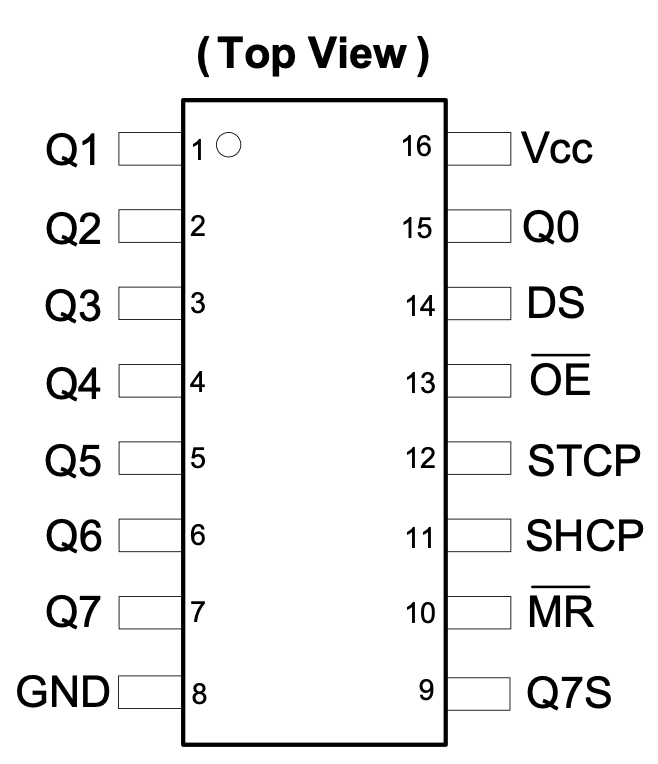
\includegraphics [width=\textwidth] {img/Schieberegister}
\end{minipage}
\begin{minipage}{0.6\textwidth}
	//TODO Ausgänge und so erklären
\end{minipage}
\newline


\subsection{Transistor}
Durchlaufspannung, Mindestspannung

\subsection{Schaltplan}

\subsubsection{Arduino}

Im Zentrum der Schaltung steht der Mikrocontroller (hier: Arduino Uno R3).
Dieser erhält Daten und Strom über den integrierten USB-Anschluss, welcher mit dem Computer verbunden wird.
Da der Arduino limitierte~\nameref{PWM}-fähige Ausgänge bereitstellt, werde Schieberegister (74HC595) verwendet.
Mit jedem ``in Reihe'' geschaltetem Schieberegister kann die Anzahl PWM-fähiger Ausgänge um 8 erweitert werden.

\subsubsection{Schieberegister}

Der Arduino wird an fünf Stellen mit dem ersten Schieberegister verbunden:

Arduinoport D2 <-> Serial (SER) Input

Über diese Verbindung werden serielle Daten werden hier bitweise in das Register geschoben.

Arduinoport D3 <-> SHCP (Shift Register Clock Input)

Dieser Pin wird verwendet, um den Takt für das Verschieben der Daten innerhalb des Schieberegisters anzulegen.
Bei jedem Taktimpuls auf diesem Pin wird das Bit am seriellen Dateneingang in das Register verschoben.
Das bedeutet, dass bei jeder steigenden Flanke des Taktsignals das Datenbit, das am Eingang anliegt, in das Schieberegister übernommen und alle vorhandenen Daten um eine Position verschoben werden.

Arduinoport D4 <-> STCP (Storage Register Clock Input)

Nachdem die Daten in das Schieberegister eingelesen wurden, wird dieser Pin verwendet, um die im Schieberegister vorhandenen Daten in das Ausgangsregister zu übertragen.
Ein Taktimpuls auf diesem Pin bewirkt, dass die Daten vom Schieberegister ins Ausgangsregister übernommen werden, sodass alle Ausgänge gleichzeitig aktualisiert werden.
Das ist besonders relevant, da sonst unter Umständen alle Ausgänge von einer Änderung im letzten Schieberegister bedingst wären.

Arduino GND <-> Ground, Output Enable (OE)

Der OE-Pin wird genutzt, um die Ausgänge des Schieberegisters global zu aktivieren oder zu deaktivieren, ohne die Daten selbst zu beeinflussen.
Da das Schieberegister zu keiner Zeit deaktiviert sein soll, wird dieser Pin dauerhaft mit dem GND-Pin verbunden.

Arduino VCC 5V <-> VCC, $\overline{SRCLR}$ (Reset)

Um das Schiebregister mit den benötigten 5V zu betreiben, wird der entsprechende Pin mit dem 5V Output des Arduino verbunden.
Zusätzlich wird der $\overline{ }$ SRCLR Port des Schieberegisters, welcher ein Reset ermöglicht dauerhaft mit 5V verbunden.

Jedes weiteres Schieberegister greift die oben genannten Signale ab.
Der einzige Unterschied befindet sich am Serial (SER) Input Port.
Das Schieberegister an Position i+1 wird mit dem seriellen Output des Schieberegisters an Position i verbunden. ($\forall i = 0,...,10$)

\subsubsection{MOSFET}

Die Hubmagnete werden jeweils mit 24V und mit bis zu 400mA betrieben.
Um einen hohen Stromfluss zu steuern, können Transistoren verwendet werden.
Für hohe Spannungen und schnelle Schaltvorgänge eigenen sich besonders MOSFETs (Metall-Oxid-Halbleiter-Feldeffekttransistor).
Im Folgenden werden speziell n-MOSFETs verwendet, der mit einem Signal zwischen 0V (leitet nicht) und +5V (voll leitend) angesteuert werden kann.

Der folgende Aufbau ist für die insgesamt 88 Ausgänge der 11 Schieberegister identisch, da jeder Ausgang für die Ansteuerung genau eines Motors zuständig ist.

Der GATE-Pin des MOSFETs erhält das Signal, dass die ``Durchlässigkeit'' steuert aus einem der Outputs des Schieberegisters.
Der SOURCE-Pin wird mit Ground des gesamten Systems verbunden.
Der DRAIN-Pin wird direkt mit dem entsprechenden Kontakt am Hubmagneten verbunden.

\subsubsection{Hubmagnet}

Um den Stromkreis zu schließen wird der andere Kontakt des Hubmagnetes mit dem +24V verbunden.

\subsubsection{Testen}

Um die Fehlersuche zu erleichtern, werden LEDs in den Schaltplan mit eingebaut.
Diese werden jeweils mit einem entsprechenden $1k\Omega$ Widerstand parallel zu den Motoren angeschlossen.
So kann anhand der Helligkeit der LED die Intensität abgelesen werden, mit der eine Taste gespielt wird.

//Bild vom Schaltplan


\section{Weitere Ideen und Limitationen}

Im Laufe der Konzeption traten mehrere Herausforderungen auf, welche aus Zeit- und Konsten- Gründen nicht weiter
behandelt wurden.
\paragraph{Anzahl der Aktuatoren}
Wie bereits erklärt, wurden insgesamt 88 Aktuatoren verbaut, womit jede Taste angespielt werden kann. Trotz der Anzahl an
Hubmagneten, werden maximal 10 Tasten glechzeitig angespielt. Dies liegt an der Stromversorgung. Ein Hubmagnet benötigt
eine Stromversorgung von etwa 0.4 Ampere, für 10 Aktuatoren sind das also 4 Ampere. Das Netzteil welches wir verwenden, ist auf
6(?) Ampere ausgelegt, wobei wir mit einem Netzteil getestet haben, welches 2,8 Ampere unterstützt. Es gibt Netzteile die
einen höheren Stromföuss ermöglichen, allerdings sind diese um weiten teurer als das Netzteil, für welches wir uns entschieden haben.
Es wäre auch möglich, ein zweites Netzteil parallel zu Schalten, wodurch die Kosten nicht dramatisch gestiegen wären.
Wir haben hier allerdings keinen Mehrwert mehr gesehen. Die Logik und Ansteuerung des Klaviers bleibt die gleiche, weswegen
wir bei einem Netzteil mit einem maximalen Stromfluss von 6 Ampere (und 24V Leistung) verblieben sind.

\paragraph{Pedalansteuerung}
Ein Klavier hat normalerweise zwei oder drei Pedale, welche die Dynamik und den Klang des Klaviers beeinflussen.
Diese sind schwerer anzuspielen als die Tasten und benötigen somit Leistungsfähigere Aktuatoren als wir für die Tasten nutzen.
Es gab eine Überlegung diese Aktuatoren zu besorgen, da die Pedale klangtechnisch Mehrwert bringen.
Außerdem hätten wir uns noch Gedanken bezüglich der Schaltug und des Signals machen können.
Einerseits hätte ein weiteres Schieberegister genutzt werden können, wobei das Signal angepasst wird das die letzten 6 Ausgänge nie ein Signal bekommen.
ANdererseits hätten die Pedale mit weiteren PWM Ports des Arduinos verbunden werden können und die Signale unabhängig von den
Schieberegistern erhalten können.
Im Prinzip wäre die Idee hier allerdings wieder die selbe wie beim Rest des Projektes gewesen,
weswegen wir Kosten an den Aktuatoren und der extra Stromversorgung für die Pedale gespart haben und diese nicht ansteuern.

\paragraph{Wärmeabfuhr}
Metallplatte unter Aktuatoren